
%%% Local Variables: 
%%% mode: latex
%%% TeX-master: t
%%% End: 

\chapter{相关工作}
\label{chap:background}

随着互联网应用需求的不断增长,数据中心所需要的服务器数量也在飞速增长中。
受到电力供应、冷却系统以及占地面积等客观因素的影响,
服务器规模并不能够无限制的扩大,即将成为数据中心发展的瓶颈;
另一方面,当前的数据中心设计并不是最优的,
典型表现在其6\%$\sim$12\%极低的资源利用率,
通过改进数据中心设计,提高服务器资源利用率,是解决数据中心扩展性问题的一个途径。
资源共享是提高资源利用率的主要手段,但它也会带来应用服务质量下降的问题,
现有大量研究尝试解决资源利用率与应用服务质量相冲突的问题,
本节对这些相关工作进行介绍。

\section{服务器资源共享}

通过服务器资源共享,将多个应用运行在同一服务器,是提高服务器资源利用率最为直接的方式。
但不同应用对操作系统、运行时环境等需求各不相同,无法直接实现应用混合部署;
即使是运行时环境兼容的2个应用,部署在同一台服务器后,
对某一应用配置的修改都可能会对另一个应用的运行造成影响;
同时,由于数据中心应用来自于不同的用户,混合部署还可能存在隐私与安全性问题,
造成应用数据信息的泄漏。
为解决以上问题,数据中心需要提供一种有效的资源隔离技术,
通过将应用运行在相互隔离的环境中,实现安全可靠的混合部署。
在服务器领域,当前流行的虚拟化与容器技术提供了这样的隔离环境。

% 虚拟化
虚拟化技术最初由IBM在20世纪60年代提出,
当时提出虚拟化的目的是为了提供系统的向后兼容性,以简化用户编程,
而后虚拟化一直是大型机基本的使用方式。
在此基础上IBM提出了逻辑分区(LPAR)\cite{IBM_LPAR:2007}技术,
该技术使得1台计算机能够像2台或更多台独立计算机一样运行,
提供了硬件层次的隔离,
其他一些厂商如Hitachi\cite{hitachi-lpar}和Sun(Oracle)\cite{LDom}也提供了类似的解决方案。

VMware最先将虚拟化技术引入到基于x86的PC服务器领域,
由于当时x86架构并没有提供任何虚拟化的支持,
VMware使用二进制翻译\cite{vmware-compare-hw-sw:2006}
的方式实现操作系统内核中不支持虚拟化的指令执行,
如图\ref{fig:compare-of-virt}(a)所示,实现对用户操作系统透明的虚拟化方案。
这种基于二进制翻译的全虚拟化方案性能存在问题,
因此Xen提出了半虚拟化(para-virtualization)\cite{barham_xen_2003}的概念,
通过修改客户机操作系统,直接使用Hypercall的方式调用Hypervisor
(如图\ref{fig:compare-of-virt}(b)所示),提高系统性能。
在虚拟化产业发展起来后,各个硬件厂商分别推出新的硬件功能以更好的支持虚拟化,
如Intel的VT-x技术和AMD的AMD-V技术,如图\ref{fig:compare-of-virt}(c)所示,
硬件辅助虚拟化逐渐成为主流。
随着虚拟化技术性能的不断提高,当前在PC服务器领域,
虚拟化技术已经成为数据中心内被普遍使用的技术。

\begin{figure}[t]
  \centering
  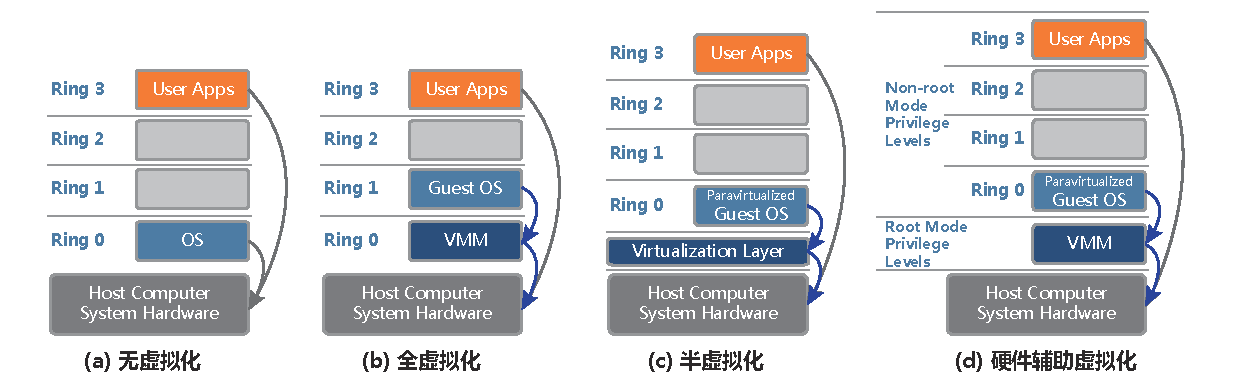
\includegraphics[width=\textwidth]{bg/compare-of-virtualization}
  \caption[3种不同类型虚拟化技术的对比]{3种不同类型虚拟化技术的对比:
    (a)无虚拟化,直接执行用户与OS请求;
    (b)全虚拟化,直接执行用户请求,二进制翻译执行OS请求;
    (c)半虚拟化,直接执行用户请求,修改GuestOS通过Hypercall实现特权指令;
    (d)硬件辅助虚拟化,直接执行用户请求,硬件支持OS特权指令直接陷入到VMM。}
  \label{fig:compare-of-virt}
\end{figure}

%容器轻量级虚拟化
基于容器的轻量级虚拟化是另一种流行的服务器融合技术,
与虚拟机抽象类似,不同容器之间以及容器与主机操作系统之间是相互隔离的,
但它们共享一份操作系统内核,可以有效的提高资源利用率。
以Docker为例(如图\ref{fig:docker-overview}),
用户应用与所依赖的运行时环境被打包为一个容器,
容器之间使用Linux内核的LXC\cite{lxc}机制实现名字空间隔离,
同时使用Control Group\cite{cgroup}实现资源控制。
与虚拟化技术相比,容器技术最大的优点是它具有更少的资源占用,以及更快的启动时间,
因此也被普遍运行在数据中心场景中。

\begin{figure}[htb]
  \centering
  \begin{minipage}{0.75\textwidth}
    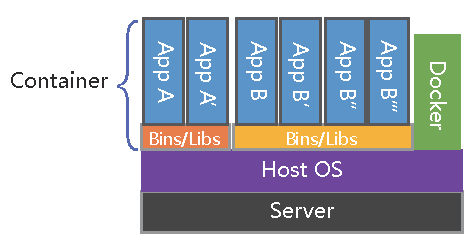
\includegraphics[width=0.75\textwidth]{bg/docker-overview}
    \caption[容器虚拟化结构示意(Docker)]{容器虚拟化结构示意(Docker):
      容器中包含应用及其依赖的运行时环境,容器之间相互隔离但它们共享同一份操作系统内核。}
    \label{fig:docker-overview}
  \end{minipage}
\end{figure}

% TODO:各种服务器融合技术对比

Google是最早在其数据中心实现多应用混合部署,他们的混合部署方案是基于cgroup的容器技术。
前文所提到的Google将离线数据中心资源利用率提高到75\%,
应用混合部署在其中起到了关键作用。
资源共享能够提高利用率,但它也带来了应用之间由于资源竞争产生的干扰。
一些研究发现,在压力测试的场景下,
现有的虚拟化技术并不能隔离异常虚拟机\cite{Matthews:2007},
这可能会对正常虚拟机的执行造成严重的影响。
另一个研究\cite{Reddy:2014}对虚拟机和真机的性能差别进行测试,
其结果如图\ref{fig:reddy-vmm-eval}所示,
即使是虚拟化开销最小的VMWare ESXi也会给程序带来平均5.4\%的性能下降,
性能下降最严重的Encryption benchmark甚至有18\%的性能下降;
Xen和KVM平均也分别有8.8\%和19.8\%的性能下降。
这也是为什么Google并没有在其在线应用数据中心采取基于虚拟化的资源共享方案的原因。

\begin{figure}[tb]
  \centering
  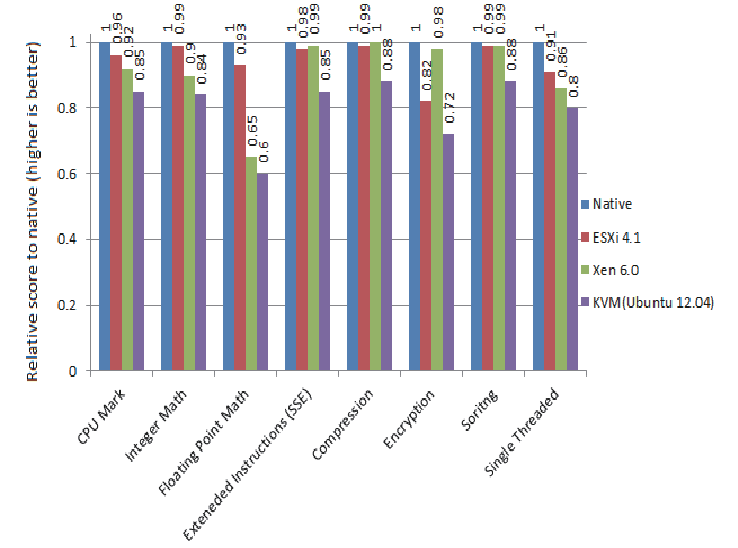
\includegraphics[width=0.8\textwidth]{bg/reddy-vmm-eval}
  \caption{不同Hypervisor性能对比\cite{Reddy:2014}}
  \label{fig:reddy-vmm-eval}
\end{figure}


另一方面,
IBM在其SoftLayer云平台中对采用虚拟机与物理机运行3年web应用后的成本与性能进行统计\cite{Stadtmueller:2015},
结果如表\ref{tab:ibm:vmm-eval}所示。
可以看到虚拟化技术虽然节省基础设施开销,但却带来额外的软件费用与性能下降,
使得单位负载开销反而高于物理机上直接部署应用。
当前虚拟化技术并不是非常完善的资源隔离技术,仍有改进空间。

\begin{table}[t]
  \centering
  \begin{minipage}[t]{0.8\linewidth}
  \caption{在IBM SoftLayer平台上运行web应用的3年成本与性能对比\cite{Stadtmueller:2015}}
  \label{tab:ibm:vmm-eval}
  \begin{tabular*}{\linewidth}{p{0.25\textwidth}<{\centering}p{0.3\textwidth}<{\raggedleft}p{0.3\textwidth}<{\raggedleft}}
    \toprule[1.5pt]
                       & \textbf{使用虚拟化技术} & \textbf{不使用虚拟化技术} \\
    \midrule[1pt]
    基础设施	       &                \$34,746 &                  \$51,840 \\
    数据传输(Internet) &                \$62,366 &                  \$68,609 \\
    软件费用	       &               \$137,760 &                  \$48,216 \\
    成本总计	       &               \$234,872 &                 \$168,665 \\
    最大RPS	       &                  19,833 &                    21,765 \\
    平均RPS	       &                   3,314 &                     3,628 \\
    单位负载开销       &                \$71/RPS &                  \$46/RPS \\
    \bottomrule[1.5pt]
  \end{tabular*}
  \end{minipage}
\end{table}

%
%\section{服务质量评价指标}
%
%性能下降程度,BubbleUP
%

\section{软件服务质量保障技术}

软件服务质量保障是指在不修改硬件的前提下,仅使用软件技术实现应用服务质量保障的方法。
按照其实现原理可以为分3类,分别是基于任务调度、资源分配和执行控制,
本节将对这3类相关工作进行介绍。

\subsection{任务调度}

数据中心中任务众多,它们有着不同的需求,虽然前文提到应用共享资源可能会产生竞争,
但也存在2个应用之间的资源需求是正交的可能,即两者之间不会发生竞争或竞争并不激烈,
在这样的情形下,资源共享并不会带来干扰。
以图\ref{fig:apps-corun-bubbleup}和图\ref{fig:apps-corun-measuring}为例,
并非所有的应用组合都会产生严重的性能干扰,例如:
图\ref{fig:apps-corun-bubbleup}中websearch与map、protobuf和sawzall三个应用混合运行时,并不会对其性能造成严重的影响;
图\ref{fig:apps-corun-measuring}中java与其中5个应用混合运行时,性能也没有出现明显的变化。
任务调度方法即是通过在应用中选择干扰较小的组合进行应用的混合部署,以实现应用服务质量保障。

\begin{figure}[tb]
\begin{minipage}[b]{0.48\textwidth}
  \centering
  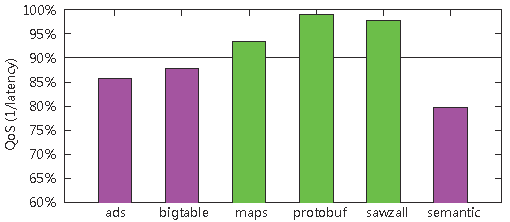
\includegraphics[width=\textwidth]{bg/apps-corun-bubbleup}
  \caption{不同应用对websearch QoS的影响\cite{mars_bubble-up:_2011}}
  \label{fig:apps-corun-bubbleup}
\end{minipage}\hfill
\begin{minipage}[b]{0.48\textwidth}
  \centering
  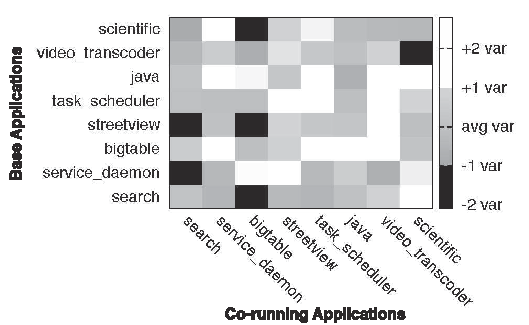
\includegraphics[width=\textwidth]{bg/apps-corun-measuring}
  \caption{数据中心应用混合运行干扰情况\cite{kambadur_measuring_2012}}
  \label{fig:apps-corun-measuring}
\end{minipage}
\end{figure}

要实现任务调度,首先需要了解应用对资源访问的行为,并对应用之间可能存在的干扰进行判断。
之前一些工作\cite{Blagodurov:2010, Chiang:2011, herdrich_rate-based_2009, Jiang:2008,
Kim:2004, mars_contention_2010, Nathuji:2010, Tang:2011}
通过在隔离的机器上运行应用获得其基准性能,
然后再与其他应用混合运行得到其性能下降,以此来获得应用之间的干扰情况。
该方法的主要问题在于其离线分析的方式只能对行为稳定、长时运行的应用有效,
而数据中心应用具有多样性,而且存在大量短作业,无法使用该方法进行干扰预测。
同时该方法在扩展性方面也存在问题:当应用数量$N$增加时,
需要进行的实验次数是以$O(N^2)$复杂度增长的,这在数据中心海量应用的场景下并不适用。

另一些研究使用共享内存资源访问的激烈程度对应用进行分类,
并以此为依据进行任务调度\cite{Chandra:2005, Knauerhase:2008, mars_contention_2010,
Zhuravlev:2010},该方案将复杂度降低到$O(N)$,
其代价是降低了干扰预测的精度,这些工作通常只能对应用进行粗略的分类,
例如划分为``激烈''与``不激烈''2类,
而不能精确的预测出2个应用混合后会出现何种程度的性能下降。
而精确的干扰预测对于任务调度来说是十分必要的,基于此需求,
Bubble-Up\cite{mars_bubble-up:_2011}提出一种精确预测2个应用混合运行后性能干扰程度的方法,
如图\ref{fig:bubble-up-overview}所示,该方法分为2部分:
1)评估不同内存子系统压力下的应用性能下降程度,以敏感曲线(sensitivity curve)表示;
2)评估应用对内存子系统产生的压力,以压力参数(pressure score)表示。
通过以上2组参数,即可量化的描述应用与内存子系统之间的关系。
通过应用B的压力参数查询应用A的敏感曲线,
即可精确的得出2个应用混合运行后的应用B对应用A性能干扰情况,
以此为指导实现QoS-aware的任务调度策略。
Bubble-Up虽然解决的扩展性与精确预测的问题,但它依然是基于离线分析的方式,
无法直接应用在数据中心场景,只能应用在负载相对稳定的场景。

\begin{figure}[tb]
  \centering
  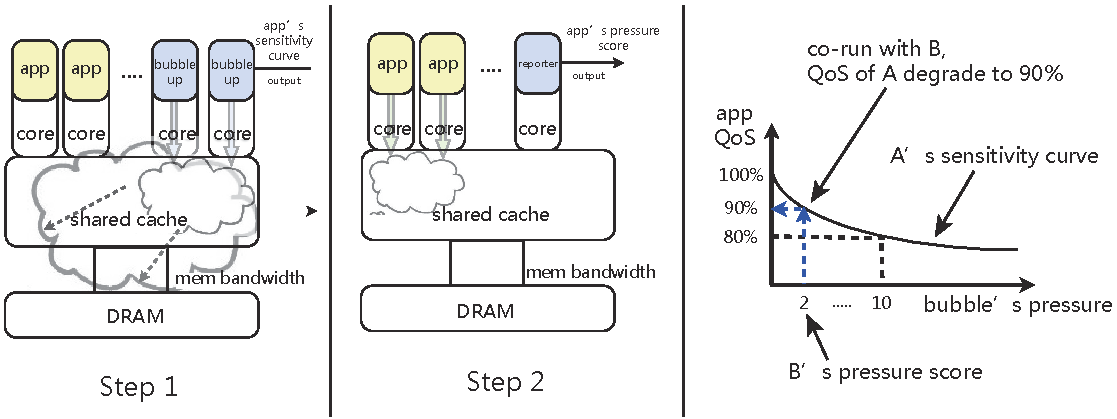
\includegraphics[width=\textwidth]{bg/bubble-up-overview}
  \caption[BubbleUp原理示意图\cite{mars_bubble-up:_2011}]{
    Bubble-Up\cite{mars_bubble-up:_2011}原理示意图:
    1)评估应用性能对内存子系统压力的敏感曲线;
    2)识别应用对内存子系统产生的压力;
    3)使用以上2组参数,识别应用之间的干扰程度。}
  \label{fig:bubble-up-overview}
\end{figure}

针对在线的应用干扰分析需求,
Kambadur等人提出了一种数据中心范围内实时干扰评估方法\cite{kambadur_measuring_2012},
其流程如下:
1)通过性能收集工作实时采集数据中心服务器性能指标并汇总;
2)使用基于统计的性能指标(如平均IPC或IPC中位数)对应用性能干扰情况进行判断;
3)利用性能采样中的时间戳信息,获取应用混合运行情况;
4)综合2)和2)的结果,对应用之间的干扰进行分类。
该方法最终得到的干扰分类信息,是实时的、数据中心全局范围的应用干扰情况,
可以作为任务调度系统执行任务调度与迁移的依据。

以上方案都是基于性能收集与分析实现应用干扰预测,
通常需要周期性的进行性能收集,才能得到准确的干扰情况。
数据中心应用具有一定的相似性和可重复性,
基于该特征Paragon\cite{delimitrou_paragon:_2013}通过器学习分类的方式,
实现应用特征的快速识别。
Paragon的分类引擎利用历史应用的调度信息进行离线训练,
建立模型识别新应用对其它应用干扰、以及新应用受到其它应用干扰的情况,
并据此实现类似推荐系统的任务调度。
其具体流程如图\ref{fig:paragon-overview}所示,首先建立应用分类模型,
当新应用到达时,利用该模型预测其行为,
包括Heterogeneity scores和Interference scores 2部分;
利用此信息进行服务器选择,完成任务调度。

\begin{figure}[tb]
  \centering
  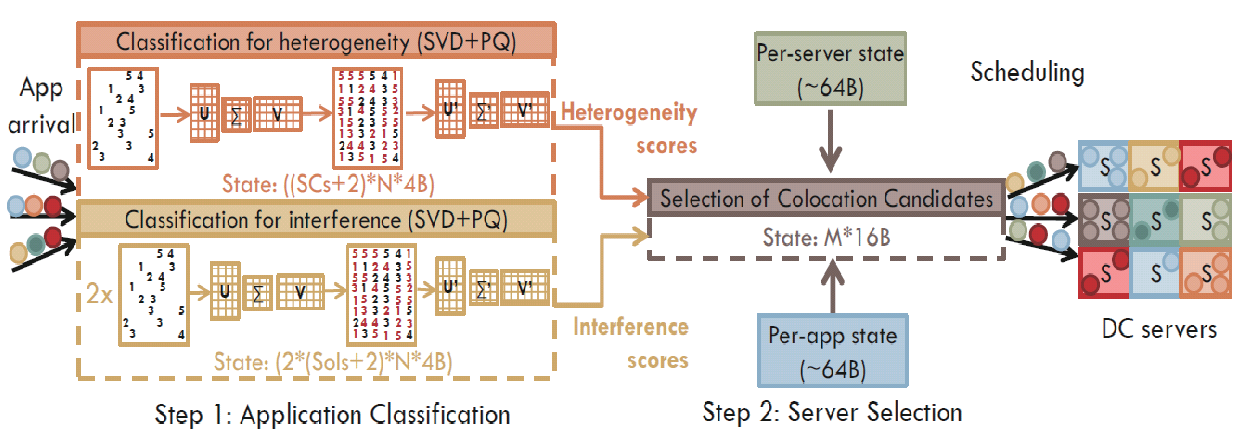
\includegraphics[width=\textwidth]{bg/paragon-overview}
  \caption{Paragon原理示意图\cite{delimitrou_paragon:_2013}}
  \label{fig:paragon-overview}
\end{figure}


\subsection{执行控制}
%ReQoS, DVFS, Bubble-Flux

上节介绍的基于任务调度的方法,
其解决资源利用率与服务质量冲突的问题所依赖的前提是存在大量可供调度的应用,
且存在干扰较小的应用组合,其利用率提高的上限取决于这样的应用组合的数量。
如果干扰较小的应用组合数量较少,或一些存在干扰的应用必须混合运行时,
基于调度的方法无法发挥其作用。

\begin{figure}[b]
  \centering
  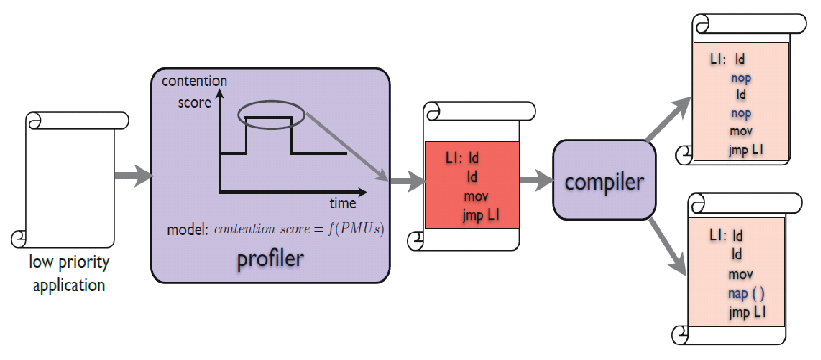
\includegraphics[width=0.8\textwidth]{bg/qos-compile-overview}
  \caption{QoS-Compile原型示意图\cite{tang:2012}}
  \label{fig:qos-compile-overview}
\end{figure}

针对该问题Tang等人\cite{tang:2012,tang_reqos:_2013}提出了另一种思路:
通过混合运行不同优先级的应用提高资源利用率,同时直接对应用之间的竞争进行管理,
以保障关键应用的服务质量。
QoS-Compile\cite{tang:2012}的流程如图\ref{fig:qos-compile-overview}所示,
首先利用编译的手段识别出应用中可能会引起内存子系统竞争的代码段,
在编译后的代码中,在这些位置增加额外的指令降低访存速率。
其提供了2种降低访问速度的方案,分别是padding和nap insertion,
前者通过在连续访存指令之间增加空指令,后者是则在访存循环中增加停顿,
这2种方式都可以降低访存速率,并以此来降低对其它应用的干扰。
对低优先级应用进行以上静态的修改,将其转换为``无干扰''的应用,
与其它高优先级的应用混合,达到提高到利用率同时保障高优先级应用服务质量的目的。

该方案的主要存在3个方面的问题:
首先,通过静态编译的方式控制低优先级应用执行的策略过于保守,
因为编译检测到的干扰点不一定会对所有其它高优先级应用造成干扰; 
其次,静态编译后的低优先级应用,无法预测其干扰的降低程度,
因此也就无法预测与其混合运行的高优先级应用的性能。
再次,对不同的应用组合,需要对低优先级应用的编译参数进行调整并重新编译,
使用不灵活。
为解决以上3个问题,ReQoS\cite{tang_reqos:_2013}对QoS-Compile方案进行了改进,
使用基于反馈的动态调整机制替代静态编译,如图\ref{fig:reqos-overview}所示。
ReQoS的编译器RQ-Compiler在竞争代码段中插入hook,而不是静态的控制指令,
该hook由运行时环境RQ-Runtime控制,在必要的时候插入适当的延迟,
根据高优先级应用当前的QoS状态控制低优先级应用的执行。

\begin{figure}[tb]
\begin{minipage}[b]{0.42\textwidth}
  \centering
  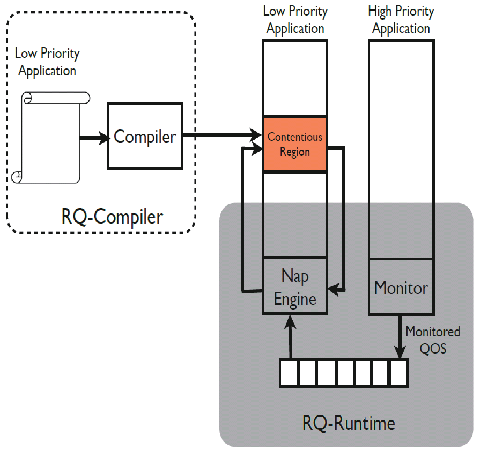
\includegraphics[width=\textwidth]{bg/reqos-overview}
  \caption{ReQoS原理示意图\cite{tang_reqos:_2013}}
  \label{fig:reqos-overview}
\end{minipage}\hfill
\begin{minipage}[b]{0.55\textwidth}
  \centering
  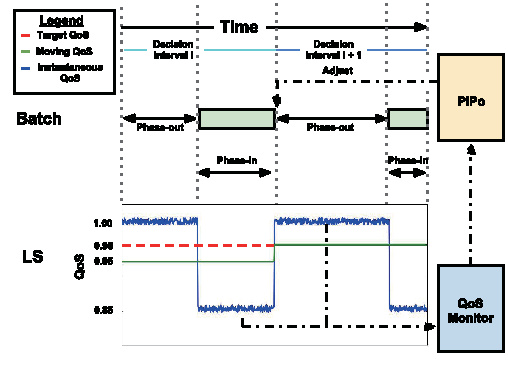
\includegraphics[width=\textwidth]{bg/bubble-flux-pipo}
  \caption{Bubble-Flux PiPo示意图\cite{yang_bubble-flux:_2013}}
  \label{fig:bubble-flux-pipo}
\end{minipage}
\end{figure}

Bubble-Flux\cite{yang_bubble-flux:_2013}也采用了直接控制竞争来防止干扰发生。
其竞争控制由Flux Engine中的QoS Monitor和PiPo(phase-in/phase-out)机制完成,
phase-out利用Linux的SIGSTOP信号暂停目标进程,
phase-in与之相反,使用SIGCONT信号启动被暂停的进程。
QoS Monitor监控高优先级应用的执行,当发生QoS违例时,
启动phase-out机制暂停低优先级应用,当干扰消除、高优先级应用QoS恢复后,
使用phase-in机制恢复低优先级应用执行。
使用PiPo机制还可以实现QoS的细粒度的控制,如图\ref{fig:bubble-flux-pipo}所示,
通过监控高优先级应用(LS)与低优先级应用(Batch)QoS的变化,
调整phase-in/phase-out的比例,以此控制低优先级应用的执行,
使得高优先级应用满足指定的QoS指标,
实现QoS的细粒度控制以及利用率与服务质量的平衡。

以上2个解决方案,其本质是使用source throttling的方式控制应用的执行,
并以此控制干扰的发生,实现服务质量的保障。
其他一些工作\cite{mars_contention_2010, herdrich_rate-based_2009, ebrahimi:2010}
也采取了该思路,只是在throttling方案选择上有所不同,
Mars等人\cite{mars_contention_2010}提出一种竞争感知的运行时环境CARE,
通过运行时环境实现throttling;
Herdrich等人\cite{herdrich_rate-based_2009}利用硬件提供的DVFS
(dynamic voltage and frequency scaling)与clock modulation技术实现throttling。
Ebrahimi等人\cite{ebrahimi:2010}利用throttling机制实现可配置的内存子系统,
允许系统软件为内存子系统制定公平规则,实现不同应用的服务质量保障。


\subsection{资源分配与隔离}

资源过量分配是当前数据中心利用率低下的一个重要原因,
而过量分配的动机则是由于共享环境下应用之间的干扰带来了性能的不确定性,
因此,实现资源按需分配的必要前提是提供良好的资源隔离机制。

cgroup\cite{cgroup}是最常用的软件资源隔离机制,
目前它提供了对处理器、内存、磁盘与网络带宽等资源的分配与隔离,
但其隔离效果并不明显。
虚拟化技术实现了隔离,但其性能隔离的效果也不好,之前的章节已经讨论过虚拟化场景下,
应用之间非常差的隔离性。
硬件层次上不受软件控制,是造成这一现状的主要原因。

% 页着色可以通过软件实现cache和dram的划分,但不太灵活
因此,当前一些工作尝试从软件控制共享硬件的行为,实现资源隔离,
页着色技术(page coloring)即是其中一种。
通过软件方式控制内存物理页映射,可以实现共享末级缓存与DRAM的划分,
其核心思路是通过控制地址映射信息实现硬件资源的管理。
一些研究利用该技术实现共享末级缓存划分\cite{lin_gaining_2008, tam_managing_2007}
来解决应用之间缓存竞争问题,
或在虚拟化场景下实现缓存划分\cite{Jin2009, Chen2010, Wang2012};
还有一些研究\cite{liu_software_2012}使用该技术实现DRAM的bank划分,
来消除bank级的干扰与竞争,或实现DRAM与末级缓存的协作式划分\cite{Liu:2014:ISCA}。
但该技术存在2个方面的问题:
首先,当应用负载发生变化时,需要在内核中重新组织空闲页链表并进行必要的页面迁移,
这需要非常大的软件开销;
更为严重的是,目前的处理器通常使用复杂的哈希算法实现从物理地址到cache index的映射
(如Intel的SandyBridge架构),
而这些哈希算法通常并不会公开,因此在这样的系统上实现页着色是不现实的。

% Cache容量划分
随着处理器核数不断增加,硬件层次上资源竞争带来的干扰趋于严重,
各个厂商也在其处理器中增加硬件资源的管理功能。
Intel在Xeon E5-v3系列处理器中通过Resource Director Technology(RDT)\cite{intel-rdt}
方案实现硬件资源管理,
其中的Cache Allocation Technology(CAT)功能为系统软件层提供了缓存容量划分接口。
基于这样的硬件平台,
Cook等人\cite{cook_hardware_2013}评估了缓存容量划分对混合运行应用带来的影响。
通过对多种应用进行混合,并采取适当的缓存容量划分策略,
该研究发现,在其实验场景中,缓存容量划分功能为所有的应用平均提高了60\%的性能,
同时也降低了对延迟敏感型应用的干扰(平均性能下降2\%,最差7\%)。
该研究结果同时也从侧面说明了硬件上提供细粒度的资源管理是有必要的,
特别是对于多应用混合运行的场景(如数据中心)。

% Quasar实现按需资源分配
%\textbf{TODO: fix Quasar}


\section{硬件服务质量保障技术}

与软件服务质量保障技术相比,在硬件层次能够对资源拥有更多的控制,实现细粒度的管理。
但其缺点也非常明显,相比软件修改,硬件修改的复杂度更高,同时周期也更长。
已有的硬件服务质量保障技术主要集中在Cache和Memory这2个对应用性能影响最大的资源上,
通过Cache容量划分、访存调度与划分的方式,实现应用之间的隔离,
进而实现应用服务质量保障。

\subsection{Cache上的服务质量保障技术}

命中率是评价Cache性能的主要指标,它与应用行为、缓存容量以及替换策略3个方面相关。
在多应用混合的场景下,不同应用对缓存容量的竞争是在Cache上出现性能干扰的主要原因,
本节主要从容量划分机制与容量划分策略2个角度,讨论解决缓存容量竞争的硬件服务质量保障技术。

容量划分是最直接的方案,上节中介绍的基于Intel缓存容量划分技术\cite{cook_hardware_2013}
可以降低应用混合场景下缓存层次上的竞争,提高性能。
Intel提供的是以路(way)为粒度的容量划分机制,大部分在Cache上的工作也都是基于路划分的。%\cite{}。
路划分方式在其扩展性上存在限制,由于受到功耗、面积、延迟、散热等因素的影响,
当前处理器中共享末级缓存的关联度通常不高,以Intel为为例,其处理器普遍只配置了24路组相联的共享末级缓存。
这就限制了能够划分的最大分区数,同时划分后Cache的关联度下降,也会造成性能下降。

为解决关联度扩展受限的问题,
一些工作提出通过硬件\cite{Ranganathan:2000}或软件\cite{lin_gaining_2008}的方式实现按组划分的缓存,
但它们在分区大小调整时会引入大量的数据复制开销。
而ZCache\cite{sanchez_zcache:_2010}提出了一种在保持物理路数不变的基础上实现更高关联度的缓存设计,
较为完美的解决了这一问题。
其设计基于以下观察:缓存的关联度与其物理路数无关,而是与替换时的候选数目相关。
在实现上,ZCache与skew-associative cache\cite{skewed-cache}类似,使用不同的hash函数访问不同的路。
由于一个数据块在每一路内只会存在于一个位置,因此对于缓存命中,只需要一次lookup操作。
在缓存替换时,ZCache使用与cuckoo hash\cite{cuckoo}类似的方案,
冲突的数据块可以被移动到下一个不冲突的位置;
当缓存miss发生后,在TagArray中遍历,从所有的victim block中选出最优的替换位置,
并进行一系列的数据块重定位,完成替换操作。

ZCache将缓存路与关联度解耦,为缓存容量划分提供更大的空间。
Vantage\cite{sanchez_vantage:_2011}以此为基础,实现了一种细粒度的缓存容量划分方案,
它通过匹配每个分区的插入与替换的速率实现近似恒定的缓存容量。
Vantage并没有划分全部的缓存容量,而且利用部分未划分的缓存区域来消除分区间的干扰,
通过调整未划分区域的大小,可以实现不同程度的隔离:
较小的未划分区域(5\%)能够提供中等程度的隔离,
而较大的未划分区域(20\%)则能够来带强隔离的效果。
基于该特性,Vantage能够满足不同隔离需求的应用,同时还能够保障每个分区内的关联度。

容量划分策略是多应用共享缓存时需要解决的另一个重要问题,策略分为静态划分与动态划分2类。
Stone等人提出了最优静态划分方案\cite{stone:1992},但由于需要获得应用在不同容量下的性能信息,
因此该方案只能用作评估基准,而无法应用到真实场景中。
同时应用在执行过程中,对Cache的需求会不断发生变化,
静态划分无法捕捉到这一个变化,所以动态划分的性能可能会优于``最优静态划分''。
最早的动态划分策略\cite{suh:2004}
根据最近命中的请求在cache set中的位置来估计应用当前Cache的使用情况。
而UCP\cite{qureshi_utility-based_2006}提供了一种低开销的Cache容量划分策略,
其容量划分依据是基于应用当前的实际Cache容量需求,
将容量分配给能够带来最收益(缺失率降低最大)的应用。

基于Vantage与UCP提供的缓存容量划分机制与策略,
Jigsaw\cite{Jigsaw:2013}使用软件定义Cache的方式,实现灵活的Cache划分与管理,解决多应用之间在Cache层次的干扰问题;
Ubik\cite{kasture_ubik:_2014}利用延迟敏感型应用瞬时性的特征,利用缓存容量划分的方式实现长尾延迟保障。


\subsection{内存上的服务质量保障技术}

当前系统中使用的内存控制器,其调度策略是针对单线程环境进行优化,
不能很好的满足数据中心这种多应用场景的需求。
例如典型的针对单线程优化的访存调度策略FR-FCFS,
能够满足单线程应用带宽与延迟的需求;
在多应用场景下,其先来先服务(FCFS)特性使得访存密集型的低优先级应用获得更高的调度优先级,
而非访存密集型高优先级应用会被低优先级应用阻塞,造成优先级反转。

现有工作主要从内存通道划分与公平调度策略2个方向去解决该问题。
Muralidhara等人提出了一种应用感知的内存通道划分技术MCP\cite{muralidhara_reducing_2011},
用于降低应用在内存子系统的干扰。

在公平调度方面,Nesbit等人提出了基于公平排队的访存调度策略\cite{Nesbit:2006},
它能保障无论内存控制器当前压力状态如何,每个线程都能获得其分配的访存带宽,
Akesson等人提出一种内存控制器的设计\cite{Akesson:2007},
它能够为应用提供最小带宽与最大延迟的服务质量保障。
Mutlu等人提出基于stall-time的公平调度算法\cite{mutlu_stall-time_2007},
保证不同线程访存的公平性;其后续工作\cite{mutlu_parallelism-aware_2008}
提出了批量调度的方法,在防止出现访存饥饿的同时保障线程间的公平。
与常规调度策略不同,
Bitirgen等人提出通过机器学习方法实现内存调度策略\cite{Bitirgen:2008},
以达到最大访存吞吐的目的。
Kim等人针对多内存控制器场景,
设计了一种可扩展的访存调度策略以提升系统访存吞吐\cite{kim_atlas:_2010};
他的另一个工作\cite{kim_thread_2010}提出面向thread-cluster的访存调度策略,
在其中同时考虑访存吞吐与线程间公平。

总结以上内存调度策略,它们分别面向各自不同的应用场景,采取特定的优化,
在数据中心通用场景下,任何单一的调度策略都不能满足应用需求。
因此提供统一的策略管理机制,实现运行时切换,
是解决当前内存调度策略目标场景单一的一个方案。


%\section{服务质量保障框架}
%
%因为软件知道应用需求,硬件能够对资源进行细粒度控制,QoS保障需要软硬件协同。
%在实现QoS策略与机制前,需要首先定义QoS指标。Iyer等人cite{}提出了3种QoS目标,分别是: 资源用量指标(Resource Usage Metrics,RUM),定义应用的资源使用,如Cache容量即为RUM指标;资源性能指标(Resource Performance  Metrics,RPM),定义资源性能,如Cache缺失率;整体性能指标(Overall Performance Metrics,OPM),指示程序的整体性能,如IPC。大多数早期QoS工作\cite{}都使用以IPC为代表的OPM作为QoS指标。针对数据中心场景,OPM中需要额外增加Tail-Latency指标,它是反映延迟敏感型在线应用性能的主要指标,工作如\cite{}都使用它作为QoS指标。资源利用率实际对应的是RUM指标,因此本文所要解决的问题就是实现RUM与OPM的平衡。
%
%CoQoS是目前对QoS保障框架描述最为完整的工作,其提出QoS保障要分为三个部分,分别是CoS Assignment、CoS Mapping、和CoS-Based Resource Mgmt。其中第一阶段用于,XXX;第二阶段用于XXX;第三阶段用于XXX。对比本文工作,本文所提出的PARD体系结构以逻辑域为粒度保障QoS,通过标签寄存器标记硬件请求,使用控制平面进行标签与资源分配映射,使用PRM集中式管理所有资源。
%
%在QoS保障框架方面,
%Rafique等人提出了一种操作系统驱动的缓存容量划分机制\cite{Rafique:2006:ASO},
%通过标记Cache访问请求来允许操作系统根据标记对Cache容量划分进行管理。
%Sharifi等人进一步提出了一种基于反馈的控制架构\cite{sharifi_mete:_2011},
%以实现端到端的片上资源管理。
%Ravi Iyer提出了一种保障CMP体系结构上缓存Qos的管理框架CQoS\cite{iyer_cqos:_2004},
%将QoS工作分为3个阶段,即优先级分类(Priority Classification)、
%优先级分配(Priority Assignment)和优先级实现(Priority Enforcement)。
%然而,该工作只设计了QoS保障的框架,而并没有详细描述具体策略和软硬件支持。
%后续的工作\cite{iyer_qos_2007, li_coqos:_2011, li_dynamic_2012}实现了
%基于class-of-service的QoS架构(CoQoS),通过为片上请求标记优先级的方式,
%实现基于优先级的Cache/DRAM/NoC请求调度。
%
%Heracles是最相似的,
%

\section{计算机网络与服务质量}
\label{sec:background:sdn}

服务质量问题在计算网络领域存在大量研究,从原型上来说主要分为3类。
第1类是资源过量分配,根据峰值需要分配网络资源,实现服务质量保障;
第2类是以集成服务(integrated services,IntServ)\cite{IntServ}和
区分化服务(differentiated services,DiffServ)\cite{DiffServ}
为代表的共享网络环境下的服务质量保障方法,
该方法的核心思路是在网络包中增加应用区分的标签,
可以是基于单个应用(IntServ)或基于服务类型(DiffServ),
以标签为粒度在网络链路上预留资源,实现服务质量保障。
第3类是以软件定义网络SDN\cite{SDN}为代表的可编程网络架构,
能够根据应用需求的变化,通过可编程的方式实现网络拓扑的调整,
同样能够实现服务质量保障。

当前数据中心区分在线应用与离线应用的方法,
映射到网络领域可以被看做是第1类和第2类方案的结合:
使用较粗的粒度对应用进行区分(在线、离线),
并为在线作业过量分配资源,以保障其服务质量。
从网络领域的经验来看,该方案会造成严重的资源浪费,
事实也是正是如此,数据中心只有6\%$\sim$12\%的资源利用率。
要解决数据中心资源利用率与服务质量冲突,可以从网络领域中借鉴更多的思路,
包括细粒度的应用区分、以及可编程的网络管理,
本文所提出的资源管理可编程体系结构正是基于以上思路。
通过在计算机体系结构内实现应用区分与可编程的资源管理,
来解决数据中心资源利用率与服务质量的冲突。

%\begin{figure}[tbh]
%  \centering
%  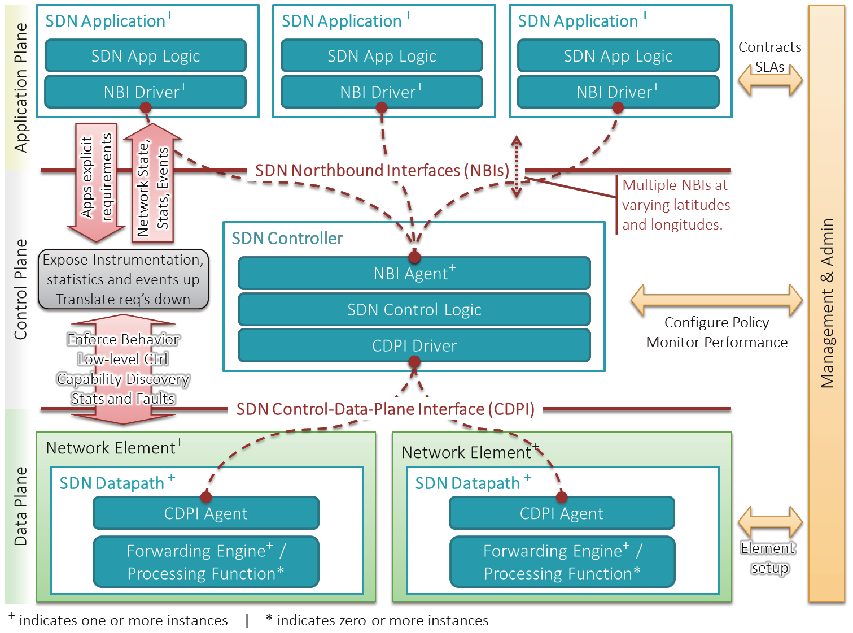
\includegraphics{arch/sdn-arch.pdf}
%  \caption{软件定义网络SDN架构}
%  \label{fig:pard-arch-outline}
%\end{figure}


\section{本章小结}

针对数据中心面临应用服务质量与资源利用率相冲突的问题,
本章从服务器资源共享和软、硬件服务质量保障机制3个角度介绍了相关研究工作。
应用之间共享资源竞争引起的性能干扰是数据中心面临问题的主要原因,
而共享的软硬件资源的竞争在整个系统栈中存在,
表\ref{tab:contention}汇总了不同层次上可能存在的竞争点,
以及在不同层次上消除竞争点的相关工作。
从现有技术来看,单节点内服务质量保障技术的不足,导致节点内应用相互干扰严重,
已经成为目前数据中心整体服务质量保障的短板,是成为长尾延迟现象的主要因素之一。
单纯从软件或硬件层次无法根本解决该问题,而是需要跨层次协同设计。
而软硬件协同设计的关键在于``应用如何表达服务质量(QoS)目标并且让底层的硬件、操作
系统以及虚拟层共同工作来保障它们''\cite{21st_architecture}。
本文后续章节将围绕该问题讨论如何设计一种新型的体系结构,
通过软硬件协同的方式解决数据中心当前面临的这一难题。

\begin{table}[tb]
  \centering
  \caption{资源管理与服务质量保障相关工作中识别出的竞争点}
  \label{tab:contention}
  \begin{tabular}{p{0.15\textwidth}p{0.75\textwidth}}
    \toprule[1.5pt]
      {\heiti 层次}     & {\heiti 竞争点}                                                                                      \\
    \midrule[1pt]
      数据中心          & Global file system \cite{dean_tail_2013}                                                                        \\
      应用层            & Background daemon \cite{dean_tail_2013}, backup job \cite{yu_profiling_2011,dean_tail_2013}                     \\
      网络协议栈        & Nagle's algorithm, limited buffers, delayed ACK caused RTO \cite{yu_profiling_2011},
                          TCP congestion control \cite{alizadeh_data_2010,dong_less_2013},
                          packet scheduling \cite{vamanan_deadline-aware_2012,wilson_better_2011,zats_detail:_2012,hong_finishing_2012},
                          kernel sockets \cite{kozyrakis_reconciling_2014}                                                                \\
      操作系统内核      & Lock contention \cite{Kapoor:2012:Chronos}, context switch, kernel scheduling,
                          SMT load imbalance and IRQ imbalance \cite{kozyrakis_reconciling_2014}                                          \\
      虚拟化层          & Virtual machine scheduling \cite{Xu:2013:Bobtail:,wang_impact_2010, Xu:2013:SMALL},
                          network bandwidth \cite{wang_impact_2010,shieh_sharing_2011,Xu:2013:SMALL,jeyakumar_eyeq:_2013}                 \\
      硬件              & Shared caches \cite{kozyrakis_reconciling_2014,Tang:2011:ISCA,kasture_ubik:_2014,sanchez_vantage:_2011,sanchez_zcache:_2010,qureshi_utility-based_2006,DelimitrouK13:ibench},
                          memory \cite{Tang:2011:ISCA,yang_bubble-flux:_2013,muralidhara_reducing_2011,DelimitrouK13:ibench},
                          NIC \cite{Radhakrishnan:2014:SENIC},
                          I/O \cite{mesnier_differentiated_2011,DelimitrouK13:ibench}                                                     \\
    \bottomrule[1.5pt]
  \end{tabular}
\end{table}



%% Comment for remove
\iffalse

\textbf{软件服务质量保障技术}\quad

在软件层次上主要采用隔离与调度2个方法实现服务质量保障。

%% 虚拟化可以提供隔离,但性能上很差,主要是硬件层次会有干扰,无法实现隔离
%虚拟化技术能够提供一定程度的
%
%

% 页着色可以通过软件实现cache和dram的划分,但不太灵活
页着色技术(page coloring)是一种以软件方式控制内存物理页映射的方法,
通常被用作共享末级缓存与DRAM的划分,其核心思路是通过控制地址映射信息实现硬件资源的管理。
一些研究利用该技术实现共享末级缓存划分\cite{lin_gaining_2008, tam_managing_2007}
来解决应用之间缓存竞争问题,
或在虚拟化场景下实现缓存划分\cite{Jin2009, Chen2010, Wang2012};
还有一些研究\cite{liu_software_2012}使用该技术实现DRAM的bank划分,
来消除bank级的干扰与竞争,或实现DRAM与末级缓存的协作式划分\cite{Liu:2014:ISCA}。
但该技术存在2个方面的问题:
首先,当应用负载发生变化时,需要在内核中重新组织空闲页链表并进行必要的页面迁移,
这需要非常大的软件开销;
更为严重的是,目前的处理器通常使用复杂的哈希算法实现从物理地址到cache index的映射
(如Intel的SandyBridge架构),
而这些哈希算法通常并不会公开,因此在这样的系统上实现页着色是不现实的。

%从调度的角度也有一些研究,但都是ad-hoc的工作,无法普及
在软件调度方面也存在大量研究,
例如,CAER框架\cite{mars_contention_2010}是一种竞争感知的轻量级运行时环境,
能在提高利用率的同时减少由于片上或片外资源的竞争所引起跨核应用之间的干扰;
CiPE框架\cite{mars_directly_2011}可以直接测量和量化多核结构下应用的跨核干扰敏感度,
并以此为依据进行作业调度。
Jason Mars等人设计的Bubble-Up\cite{mars_bubble-up:_2011}机制,
通过使用气泡(Bubble)来代表内存子系统的可变压力情况,
能准确预测在内存子系统中竞争共享资源而导致的性能下降,通过离线分析来决定最优的应用混合,
Bubble-Flex\cite{yang_bubble-flux:_2013}工作在Bubble-Up离线的基础上,实现了在线的QoS管理。
ReQoS\cite{tang_reqos:_2013}提供了一种编译技术与运行时环境相结合的方法,
通过编译的方法标识出低优先级应用中可能引起竞争的代码段,
通过运行时环境调节低应用级应用的执行来确保这些代码段不会对高优先级应用的服务质量造成影响。
以上这些工作虽然能够缓解服务质量与资源利用率的冲突,
但它们的解决方案都只能针对特定的场景,不具有通用性。


\textbf{硬件服务质量保障技术}\quad

由于单纯使用软件技术无法解决应用在硬件层次的干扰,
目前学术界和工业界在硬件层次上提出一系列方案,解决干扰问题。
其中以处理器末级缓存与内存控制器上的硬件方案居多。

针对处理器末级缓存容量的竞争,Kasture和Sanchez提出的Ubik\cite{kasture_ubik:_2014},
通过识别和利用延迟敏感型应用瞬时性的特点,调整缓存容量划分策略,来保证目标长尾延迟。
UCP\cite{qureshi_utility-based_2006}提出了一种应用缓存容量需求的探测方法,
为应用分配收益最大的缓存划分方案。
由于受到工艺、面积以及能耗的限制,目前的常见处理器末级缓存关联度最大只有24,
不足以分配给其上运行的应用,
针对该问题ZCache\cite{sanchez_zcache:_2010}提出了一种新的缓存方法,将缓存路与关联度解耦,
提高关联度为缓存容量划分提供更大的空间,
Vantage\cite{sanchez_vantage:_2011}基于该缓存设计实现了一种细粒度的缓存容量划分方案。

%Kasture and Sanchez propose Ubik \cite{kasture_ubik:_2014},
%a cache partitioning policy that characterizes and leverages the transient
%behavior of latency-critical applications to maintain their target tail latency.
%Vantage \cite{sanchez_vantage:_2011} implements fine-grained cache partitioning
%using the statistical properties of Zcaches \cite{sanchez_zcache:_2010}.
%Utility-based cache partitioning (UCP) \cite{qureshi_utility-based_2006}
%strictly partitions the shared cache depending on the benefit of allocating
%different number of ways to each application.


除硬件层次的划分与调度外,Andrew Herdrich等人\cite{herdrich_rate-based_2009}
发现了用于功耗管理的处理器限速技术(如DVFS),
能够应用到QoS领域用于实现处理器末级缓存与内存控制器上的竞争管理。
其基本方法是当正在运行的低优先级任务由于资源竞争争而干扰了高优先级任务的性能时,
就减缓核心的处理速率,通过请求抑制的方法缓解低优先级任务对共享资源的竞争。


\fi
